\documentclass{article}

\usepackage{algorithmic}
\usepackage{amsmath}
\usepackage{graphicx}
\usepackage{hyperref}
\usepackage{booktabs}
\usepackage{verbatim}

\begin{document}

\title{Final Exam}
\author{Geoffrey Ulman\\
        CSI873}
\date{December 2011}
\maketitle

\section{Implementation}\label{Implementation}

The support vector machine constrained optimization problem was modeled and solved using AMPL (\url{www.ampl.com/}). Computations were performed using the LOQO solver (\url{www.princeton.edu/~rvdb/loqo/LOQO.html}) on the NEOS server (\url{www.neos-server.org/neos/solvers/}). Once the solution to the dual problem was obtained, the \(\alpha\) values were imported into Java.

Java (version 1.6.0\_27) was used to make the final classification. The code is available as a Subversion repository on Google Code at \url{http://code.google.com/p/csi873/}. Compiling and running the code requires the Java build tool Maven (\url{http://maven.apache.org/}).

\section{Model}\label{Model}

The following AMPL model was used to solve the dual SVM problem in Equation \ref{svm} with a polynomial kernel.

\begin{equation}\label{svm}
\begin{split}
\max_\alpha \sum_{i=1}^l \alpha_i - 0.5 \sum_{i,j}^l \alpha_i \alpha_j y_i y_j K \left( x_i , x_j \right) \\
s.t. \\
\sum_{i=1}^l \alpha_i y_i = 0 \\
0 \ge \alpha_i \ge C , i = 1,2,...,l
\end{split}
\end{equation}

\begin{verbatim}

model;

# number of training examples
param l;

# number of input parameters (pixels in digit image)
param n;

# weight on xi penalty coefficient in primal problem
param C;

# parameters for polynomial machine kernel
param alpha;
param beta;
param delta;

# output vector (1 or -1)
param y { 1..l };

# input data
param x { 1..l, 1..n };

# dual problem variables and simple constraints
var a {1..l} >= 0, <= C;

maximize obj: sum { i in 1..l } a[i] - 0.5 *
              sum { i in 1..l, j in 1..l } a[i] * a[j] * y[i] * y[j] *
              ( alpha * ( sum { k in 1..n } x[i,k] * x[j,k] ) + beta ) ^ delta;

s.t. const: sum { i in 1..l } a[i] * y[i] = 0;

option solver loqo;

\end{verbatim}

The model used for the radial basis kernel was almost identical except for the objective (and some different parameters):

\begin{verbatim}

# parameters for radial basis function kernel
param gamma;

maximize obj: sum { i in 1..l } a[i] - 0.5 *
              sum { i in 1..l, j in 1..l } a[i] * a[j] * y[i] * y[j] *
              exp( -gamma * ( sum { k in i..n } ( x[i,k] - x[j,k] )^2 ) );

\end{verbatim}

\section{Two Digit Results}\label{Results2}

When the model was trained with the digit ''2`` and digit ''5`` training data, a misclassification error (on the testing data set) of \(0.098\) was achieved with the polynomial kernel and \(0.110\) with the radial kernel. The full results are summarized in Table \ref{error1}.

\begin{table}
\caption{Digit 2 vs 5 Error}
\begin{center}
\begin{tabular}{llcc}
\toprule
Data Set & Error & \multicolumn{2}{c}{95\% Confidence Interval} \\
\cmidrule(r){3-4}
& & Lower Bound & Upper Bound \\
\midrule
Polynomial Training & 0.000 & 0.000 & 0.000 \\
Polynomial Testing & 0.098 & 0.033 & 0.162 \\
Radial Training & 0.027 & 0.004 & 0.050 \\
Radial Testing & 0.110 & 0.042 & 0.177 \\
\bottomrule
\end{tabular}
\label{error1}
\end{center}
\end{table}

Figures \ref{poly2testconfusion} and \ref{radial2testconfusion} show the confusion matrices for the polynomial and radial kernels respectively. Figures \ref{radial5correcttest}, \ref{radial2correcttest}, \ref{poly5correcttest}, and \ref{poly2correcttest} display images for the correctly classified training data samples for the polynomial and radial kernels applied to the ''2`` versus ''5`` classification problem. Figures \ref{poly2errortest} and \ref{radial2errortest} display the incorrectly classified ''2`` digits for the polynomial and radial kernels. Figures \ref{poly5errortest} and \ref{radial5errortest} display the incorrectly classified ''5`` digits for the polynomial and radial kernels.

\begin{figure}
\centering
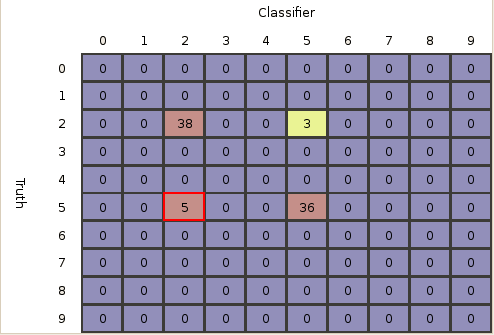
\includegraphics[width=0.9\textwidth]{images/test2_5_confusion_a0156.png}
\caption{Polynomial Kernel 2 Digit Test Error Confusion Matrix}
\label{poly2testconfusion}
\end{figure}

\begin{figure}
\centering
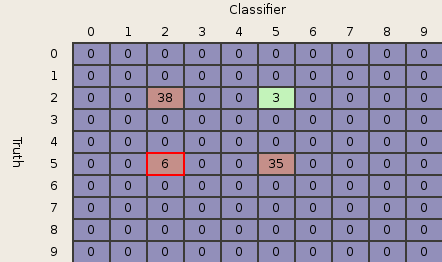
\includegraphics[width=0.9\textwidth]{images/test2_5_confusion_radial.png}
\caption{Radial Kernel 2 Digit Test Error Confusion Matrix}
\label{radial2testconfusion}
\end{figure}

\begin{figure}
\centering
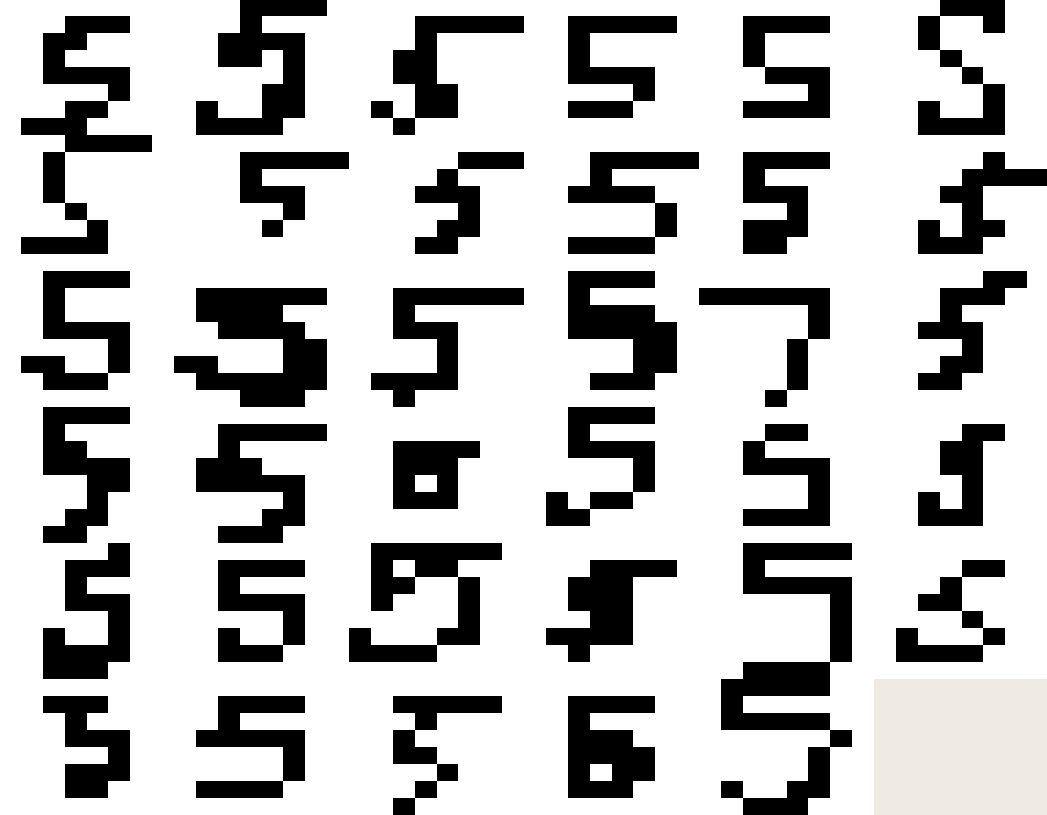
\includegraphics[width=0.9\textwidth]{images/test2_5_correct5_radial.png}
\caption{Radial Kernel Correctly Classified 5 Digits}
\label{radial5correcttest}
\end{figure}

\begin{figure}
\centering
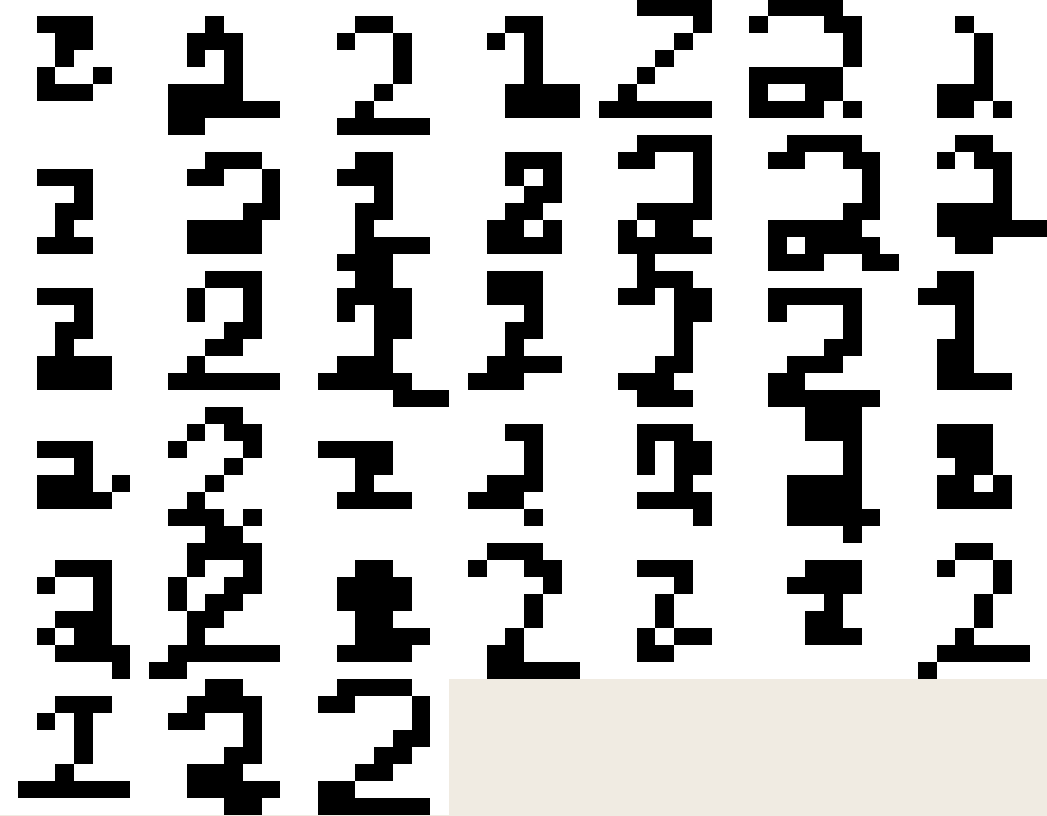
\includegraphics[width=0.9\textwidth]{images/test2_5_correct2_radial.png}
\caption{Radial Kernel Correctly Classified 2 Digits}
\label{radial2correcttest}
\end{figure}

\begin{figure}
\centering
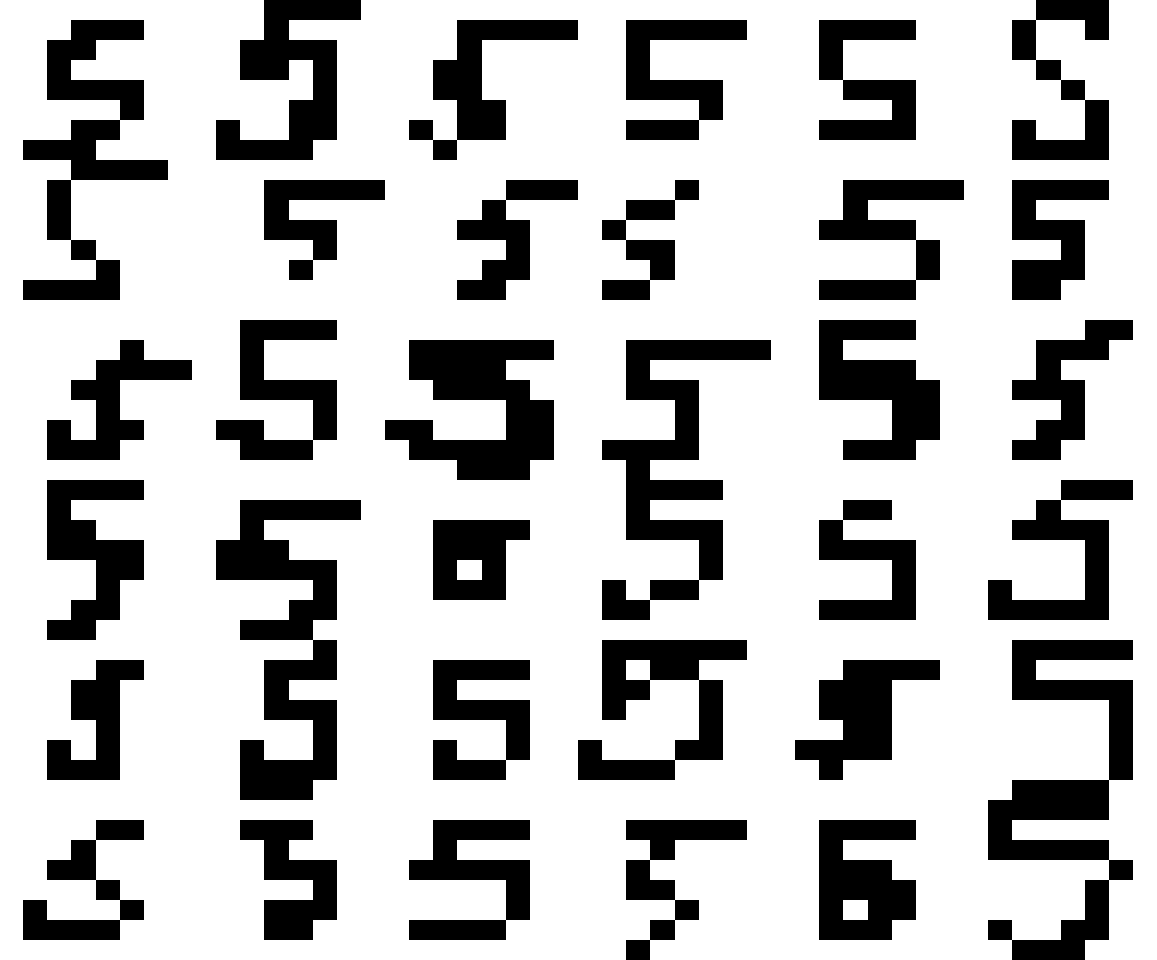
\includegraphics[width=0.9\textwidth]{images/test2_5_correct5s_a0156.png}
\caption{Polynomial Kernel Correctly Classified 5 Digits}
\label{poly5correcttest}
\end{figure}

\begin{figure}
\centering
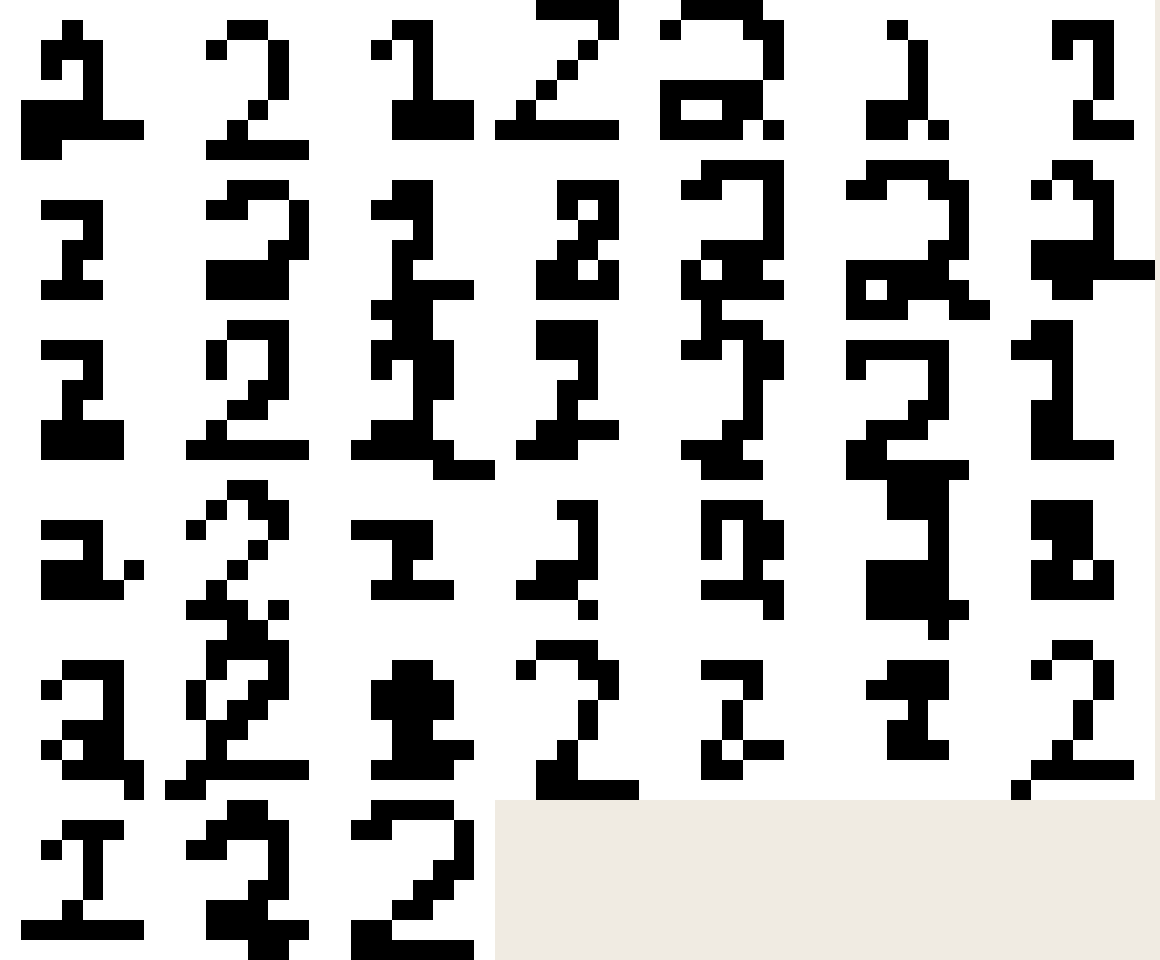
\includegraphics[width=0.9\textwidth]{images/test2_5_correct2s_a0156.png}
\caption{Polynomial Kernel Correctly Classified 2 Digits}
\label{poly2correcttest}
\end{figure}

\begin{figure}
\centering
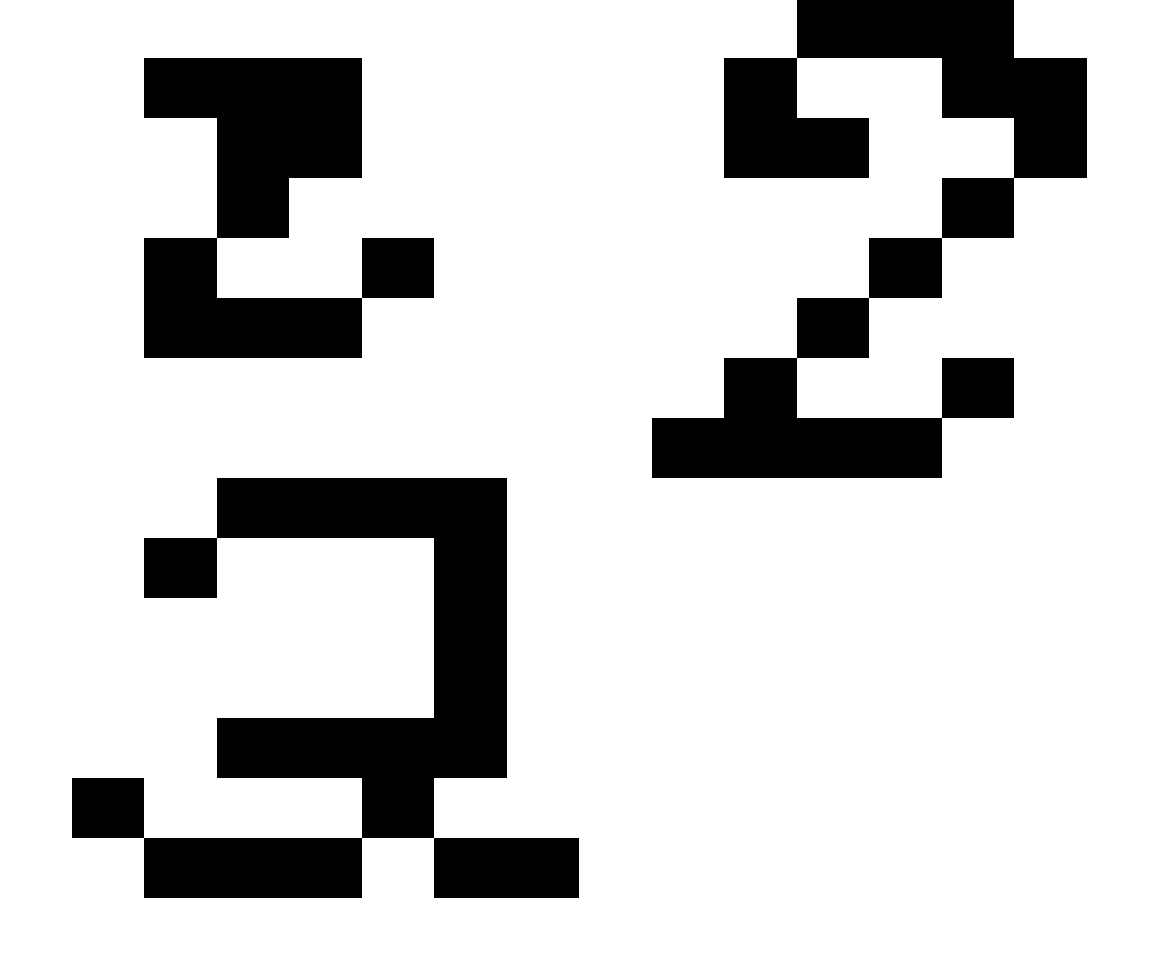
\includegraphics[width=0.9\textwidth]{images/test2_5_correct2_class5_a0156.png}
\caption{Polynomial Kernel 2 Misclassified as 5}
\label{poly2errortest}
\end{figure}

\begin{figure}
\centering
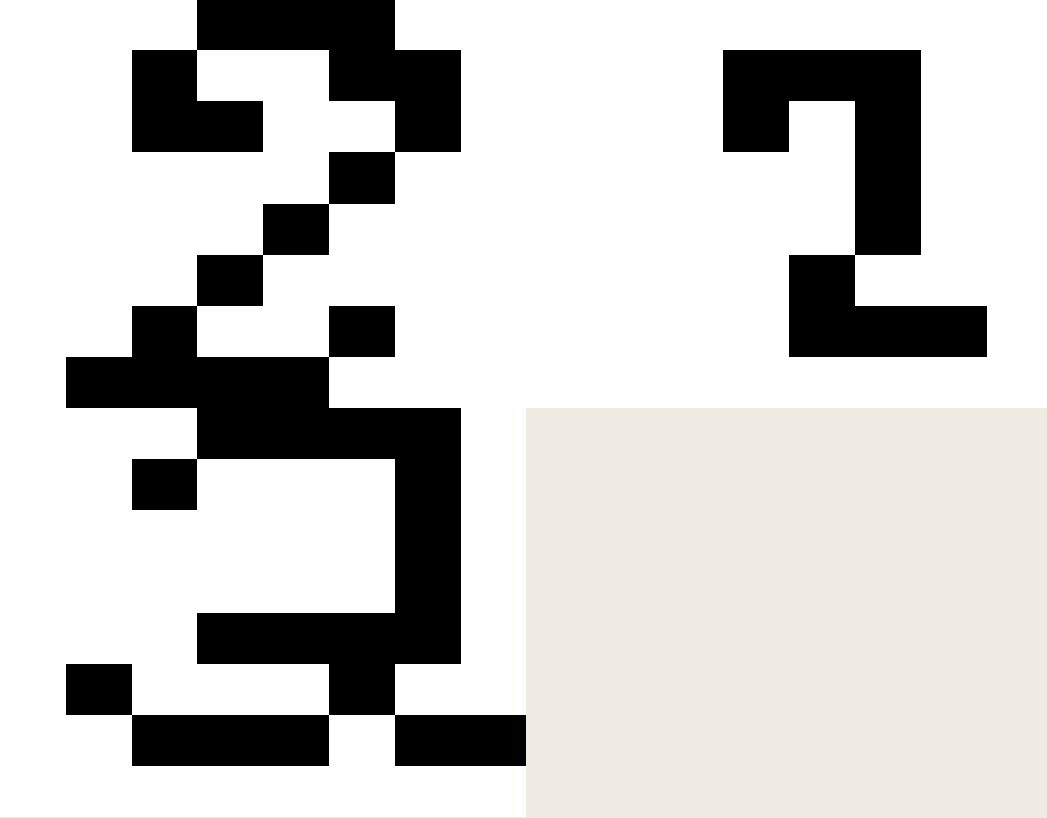
\includegraphics[width=0.9\textwidth]{images/test2_5_correct2_class5_radial.png}
\caption{Radial Kernel 2 Misclassified as 5}
\label{radial2errortest}
\end{figure}

\begin{figure}
\centering

\includegraphics[width=0.9\textwidth]{images/test2_5_correct5_class2_a0156.png}
\caption{Polynomial Kernel 5 Misclassified as 2}
\label{poly5errortest}
\end{figure}

\begin{figure}
\centering
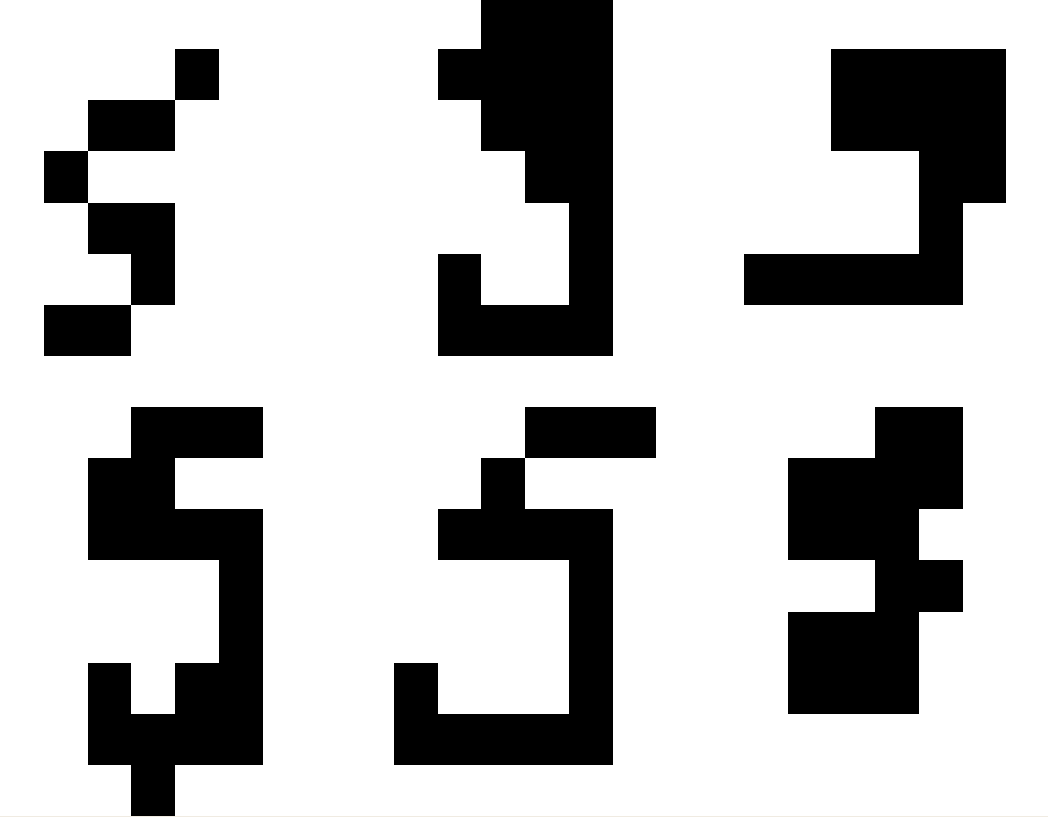
\includegraphics[width=0.9\textwidth]{images/test2_5_correct5_class2_radial.png}
\caption{Radial Kernel 5 Misclassified as 2}
\label{radial5errortest}
\end{figure}

Based on these experiments, the polynomial kernel was chosen to be used for the full problem. However, both methods performed quite well and their 95\% confidence intervals have significant overlap. So it is unclear which method is actually superior for this handwriting problem.

\section{All Digit Results}\label{ResultsAll}

A misclassification error (on the full ten digit testing data set) of \(0.200\) was achieved with the polynomial kernel. The full results are summarized in Table \ref{error2}. Figures \ref{poly10testconfusion} and \ref{poly10trainconfusion} provide confusion matrices for the testing and training data sets.

\begin{table}
\caption{All Digits Error}
\begin{center}
\begin{tabular}{llcc}
\toprule
Data Set & Error & \multicolumn{2}{c}{95\% Confidence Interval} \\
\cmidrule(r){3-4}
& & Lower Bound & Upper Bound \\
\midrule
Polynomial Training & 0.029 & 0.018 & 0.040 \\
Polynomial Testing & 0.200 & 0.161 & 0.239 \\
\bottomrule
\end{tabular}
\label{error2}
\end{center}
\end{table}

\begin{figure}
\centering
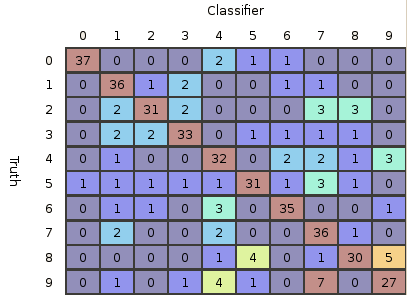
\includegraphics[width=0.9\textwidth]{images/poly_all_confusion_test.png}
\caption{Polynomial Kernel 10 Digit Test Error Confusion Matrix}
\label{poly10testconfusion}
\end{figure}

\begin{figure}
\centering
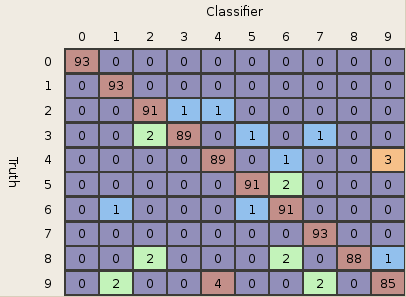
\includegraphics[width=0.9\textwidth]{images/poly_all_confusion_training.png}
\caption{Polynomial Kernel 10 Digit Training Error Confusion Matrix}
\label{poly10trainconfusion}
\end{figure}

\section{Parameterization}\label{Parameterization}

The \(\alpha_i\) upper bound parameter \(C\) was initially set at 100. Table \ref{svmcount} gives the number of support vectors (with non-zero and non-C \(\alpha_i\) value) for each of the 10 SVM optimization problems solved for the 10 digit case. Out of 930 input vectors, only about 10\% to 20\% are chosen as support vectors by the solver. This relatively low number of support vectors indicates that the choice of \(C\) as 100 was reasonable.

\begin{table}
\caption{Number of Support Vectors Out Of 930}
\begin{center}
\begin{tabular}{cc}
\toprule
Digit & Support Vector Count \\
\midrule
0 & 150 \\
1 & 121 \\
2 & 174 \\
3 & 189 \\
4 & 145 \\
5 & 216 \\
6 & 170 \\
7 & 147 \\
8 & 187 \\
9 & 155 \\
\bottomrule
\end{tabular}
\label{svmcount}
\end{center}
\end{table}

\section{Comparison}\label{Comparison}

Figure \ref{error3} provides an error rate comparison between the four major classification methods which were applied to the handwriting data set. Weighted K-Nearest Neighbors with \(k=7\) came close to the performance achieved by the polynomial kernel support vector machine (with \(0.217\) error versus \(0.200\) for the support vector machine). Naive Bayes and Neural Networks trailed with \(0.388\) and \(0.463\) misclassification error respectively.

\begin{table}
\caption{Missclassification Error Overview}
\begin{center}
\begin{tabular}{llcc}
\toprule
Algorithm & Error & \multicolumn{2}{c}{95\% Confidence Interval} \\
\cmidrule(r){3-4}
& & Lower Bound & Upper Bound \\
\midrule
Support Vector Machine & 0.200 & 0.161 & 0.239 \\
K-Nearest Neighbors & 0.217 & 0.177 & 0.257 \\
Naive Bayes & 0.388 &  0.341 & 0.435  \\
Neural Network & 0.463 &  0.415 & 0.512  \\
\bottomrule
\end{tabular}
\label{error3}
\end{center}
\end{table}

\section{Appendix}\label{Appendix}

The appendix to this report contains a number of supporting documents. The Java source code used to read the AMPL results, perform the classification, and compute statistics is included first. The code is also available at \url{http://code.google.com/p/csi873/source/browse/trunk/src/main/java/edu/gmu/classifier/svm/ampl/DataFileGenerator.java}.

Following the Java code are the AMPL model files (both with the polynomial and radial kernels) and the AMPL data file for the ''2`` versus ''5`` classification problem (the data file for the full problem is omitted due to length). However, all AMPL model, data, and NEOS output files are also available at \url{http://code.google.com/p/csi873/source/browse/#svn\%2Ftrunk\%2Ffinal\%2Fampl}.

\begin{thebibliography}{9}

\bibitem{cpl}
  Tom M. Mitchell,
  \emph{Machine Learning},
  WCB McGraw-Hill, Boston,
  1997.

\end{thebibliography}

\end{document}
